\section{Example code}
\label{sec:examples}
Possible changes to Germinate may range from basic formatting changes to the addition of completely new content. The following sections contain detailed examples for the most common scenarios of extension. Each example consists of the necessary code and accompanying explanations.

%\subsection{Adding a new page}
%This paragraph will explain how to create a basic page that contains a simple table with data from the database.
%
%\subsubsection{Creating a service}
%First, we will create a new Service which takes care of the communication between client and server. This interface contains all the methods the client can call to get data and the server has to implement.
%
%Create a new Interface called \texttt{SampleService} in the package \path{jhi.germinate.client.service}. Make it extend \path{com.google.gwt.user.client.rpc.RemoteService}. Eclipse will now tell you: "Missing asynchronous interface SampleServiceAsync". Let Eclipse create this asynchronous interface for you by selecting: "Create asynchronous RemoteService interface \texttt{SampleServiceAsync}". You will now see the new interface \texttt{SampleServiceAsync} in the same package. Now lets create some basic code that makes things easy :
%	\begin{lstlisting}[style=Java]
%/* Tells the client which relative path to use for communication with the server */
%@RemoteServiceRelativePath("sample")
%public interface SampleService extends RemoteService
%{
%    /* Create an instance of the interface that can be used to call the methods */
%    public static final class Instance
%    {
%        private static final class InstanceHolder
%        {
%            private static final SampleServiceAsync INSTANCE = GWT.create(SampleService.class);
%        }
%
%        public static final SampleServiceAsync getInstance()
%        {
%            return InstanceHolder.INSTANCE;
%        }
%    }
%}
%	\end{lstlisting}
%
%\subsubsection{Defining methods}
%Now you can define any kind of method which takes arguments from the client, sends them to the server and returns a result to the client.
%
%Let's start with a very basic method that takes an id of a specific table in the database and returns the information for that item to the client. First of all we have to define a constant in the \texttt{SampleService} interface that holds the column names of the target table. With this approach, both client and server know which data they are talking about. Add the following line to the interface:
%\begin{lstlisting}[style=Java]
%public static final String[] COLUMNS_GERMINATEBASE = { "id", "name", "number" };
%\end{lstlisting}
%As you can see, we want to get the id, the name and the number from the \texttt{germinatebase} table as the result from the service. Now lets define the method that we can call to get this data:
%\begin{lstlisting}[style=Java]
%GerminateTable getGerminatebaseData(RequestProperties properties, int id) throws InvalidSessionException, DatabaseException;
%\end{lstlisting}
%Eclipse will now tell you that "\texttt{SampleServiceAsync} is missing method \texttt{getGerminatebaseData}", which just means that there is no "partner-method" in the async interface. Let Eclipse solve this for you by selecting: "Generate method \texttt{getGerminatebaseData} in type \texttt{SampleServiceAsync}".
%
%Let's have a look at the method definition: The return type is \texttt{GerminateTable} which is a data structure we created to make the transmission of data in table structure easy. You will see how to use it later on. The parameters this method takes are the request properties (including session id and user id) and the id of the germinatebase table. The request properties \textbf{have} to be send with each request to the server. The server will then check if the transmitted session is valid (compare it to the Cookie and the server session id). This makes sure that you can't use the service without a valid session. The method throws two Exceptions. The \texttt{InvalidSessionException} is thrown if the session id is invalid and the \texttt{DatabaseException} is thrown if the interaction with the database fails in any way.
%
%\subsubsection{Database communication}
%Now the service template (interface) is set up, but the actual implementation that extracts the data from the database is still missing.
%{\sloppy %Use sloppy to force line breaks of URLs
%Now we create a class called \texttt{SampleServiceImpl} in the package \texttt{jhi.germinate.server}. This class has to extend \path{jhi.germinate.server.util.BaseRemoteServiceServlet} and implement our \texttt{SampleService}. Eclipse will now tell you that you have to implement the method \texttt{get\allowbreak Germinate\allowbreak base\allowbreak Data}. Tell Eclipse to 'Add unimplemented methods'. Now you will see something that looks like this:}
%\begin{lstlisting}[style=Java]
%@Override
%public GerminateTable getGerminatebaseData(RequestProperties properties, int id) throws InvalidSessionException, DatabaseException
%{
%    // TODO Auto-generated method stub
%    return null;
%}
%\end{lstlisting}
%Great, now all we have to do is query the database and return a \texttt{GerminateTable}. To do that, define a constant containing your SQL query, \eg:
%\begin{lstlisting}[style=Java]
%private static final String QUERY = "SELECT id, name, number FROM germinatebase WHERE id = ?";
%\end{lstlisting}
%As you can see, this query will get the id, name and number from the germinatebase table and it contains a placeholder for the id. Now lets create a connection to the database and run our query:
%\begin{lstlisting}[style=Java]
%@WebServlet(urlPatterns = {"/germinate/sample"})
%public class SampleServiceImpl extends BaseRemoteServiceServlet implements SampleService
%{
%    private static final String QUERY = "SELECT id, name, number FROM germinatebase WHERE id = ? ORDER BY id";
%
%    @Override
%    public GerminateTable getGerminatebaseData(RequestProperties properties, int id) throws InvalidSessionException, DatabaseException
%    {
%        HttpServletRequest req = getThreadLocalRequest();
%        /* Connect to the database and check the session id */
%        Database database = Database.connectAndCheckSession(properties, req);
%
%        /* Create the query and replace the placeholder (index starting from 1!) */
%        DatabaseStatement stmt = database.prepareStatement(QUERY);
%        stmt.setInt(1, id);
%        
%        /* Use the String[] we defined in the SampleService to extract the data */
%        GerminateTable result = database.runQuery(stmt, COLUMNS_GERMINATEBASE);
%        
%        /* Remember to close the database connection (may create a memory leak if you don't!) */
%        database.closeConnection();
%        
%        /* Return our data */
%        return result;
%    }
%}
%\end{lstlisting}
%As you can see, the method \texttt{Database\#runQuery(...)} will create a \texttt{GerminateTable} for you. Great, so just return it.
%
%There are two utility classes called \texttt{GerminateTableQuery} and \texttt{ValueQuery}. We can use the \texttt{GerminateTableQuery} to reduce the code we have seen to two lines (formatted for easy readability):
%
%\begin{lstlisting}[style=Java]
%@Override
%public GerminateTable getGerminatebaseData(RequestProperties properties, int id) throws InvalidSessionException, DatabaseException
%{
%    HttpServletRequest req = getThreadLocalRequest();
%    return new GerminateTableQuery( /* We use the "fluent code" class to query the database */
%                                      properties, /* Pass in the session request parameters */
%                                      this, /* and the servlet to validate the user based on the request */
%                                      QUERY, /* This is the SQL query */
%                                      COLUMNS_GERMINATEBASE ) /* This is the array of columns to extract */
%                                      .setInt(id) /* Replace the first placeholder with the id */
%                                      .run() /* finally run the query on the database */
%                                      .getServerResult(); /* We only want the table, not the debug information */
%}
%\end{lstlisting}
%\noindent
%This is basically a highly packed version of the first code to reduce clutter. That's it for the server side code.
%
%\subsubsection{Server configuration}
%So far we have taken care of the communication interface and the server implementation, but the server does not know, which requests to redirect to the implementation.
%
%Open the file \texttt{SampleServiceImpl} and add this annotation to the class:
%\begin{lstlisting}[style=Java]
%@WebServlet(urlPatterns = {"/germinate/sample"})
%public class SampleServiceImpl extends BaseRemoteServiceServlet implements SampleService
%\end{lstlisting}
%This is a mapping of a url-pattern to the servlet, \ie the server will redirect requests to the relative url \texttt{/germinate/sample} to the newly defined servlet.
%
%\subsubsection{Client GUI implementation}
%\label{sec:example_client}
%Now we defined the communication interface between client and server and the server side part. All that's missing is code on the client side to call the method and show the result.
%
%Now let's create a very simple page that contains a text field for the id, a button to send the request and a table to show the result.  Create a new class called \texttt{GerminatebaseData} in the package \texttt{jhi.germinate.client.composite.sample}. Let this class extend \texttt{com.google.gwt.\allowbreak user.client.ui.Composite}. The overall code looks like this:
%\begin{lstlisting}[style=Java]
%public class GerminatebaseData extends Composite
%{
%    /* Define an array that holds the internationalized column names */
%    private static final String[] COLUMNS_I18N = new String[SampleService.COLUMNS_GERMINATEBASE.length];
%
%    /* Fill the internationalized array */
%    static
%    {
%        int i = 0;
%        COLUMNS_I18N[i++] = Text.LANG.sampleColumnsId();
%        COLUMNS_I18N[i++] = Text.LANG.sampleColumnsName();
%        COLUMNS_I18N[i++] = Text.LANG.sampleColumnsNumber();
%    }
%
%    /* Panel that holds the result table */
%    private SimplePanel           resultPanel;
%
%    public GerminatebaseData()
%    {
%        /* Define a flow panel that will hold all our content */
%        FlowPanel panel = new FlowPanel();
%
%        /* Create the text box for the germinatebase id */
%        final TextBox baseId = new TextBox();
%
%        /* Create a button to start the server request */
%        Button query = new Button();
%        /* Add the internationalized text */
%        query.setText(Text.LANG.generalButtonContinue());
%
%        /* Create the panel that will hold the result table */
%        resultPanel = new SimplePanel();
%
%        /* Add everything to the panel */
%        panel.add(baseId);
%        panel.add(query);
%        panel.add(resultPanel);
%
%        /* Add a listener to the button */
%        query.addClickHandler(new ClickHandler()
%        {
%            @Override
%            public void onClick(ClickEvent event)
%            {
%                queryServerForData(baseId.getText());
%            }
%        });
%
%        /* Set the content of this composite to be the panel */
%        initWidget(panel);
%    }
%
%    /**
%     * This method will query the server for the data for the given query text
%     * 
%     * @param queryText
%     *            The entered query text (the id of the germinatebase table)
%     */
%    private void queryServerForData(String queryText)
%    {
%        int id;
%
%        try
%        {
%            /* See if the entered text is an integer */
%            id = Integer.parseInt(queryText);
%        }
%        catch (NumberFormatException e)
%        {
%            /* If not, notify the user that s/he should enter a number */
%            Notification.error(Text.LANG.notificationSampleNoNumber());
%            return;
%        }
%
%        /* This callback will be called when the server result returns. It will
%         * either be a success of a failure. */
%        AsyncCallback<GerminateTable> callback = new AsyncCallback<GerminateTable>()
%        {
%            @Override
%            public void onFailure(Throwable caught)
%            {
%                /* If the request failed, check the reason */
%                if (caught instanceof InvalidSessionException)
%                {
%                    /* If the session is invalid, we will show an error
%                     * notification, log the user out and clear all stored data */
%                    Notification.error(Text.LANG.notificationInvalidSession());
%                    Core.INSTANCE.setLoggedIn(false);
%                    TypedParameterStore.clearAll();
%                    History.fireCurrentHistoryState();
%                }
%                else
%                {
%                    /* Else, it will be a DatabaseException and we can just
%                     * notify the user */
%                    Notification.error(caught.getLocalizedMessage());
%                }
%            }
%
%            @Override
%            public void onSuccess(GerminateTable result)
%            {
%                /* If the query was successful, remove any previous table */
%                resultPanel.clear();
%
%                /* And create a basic table by passing the GerminateTable, the
%                 * database column names, the internationalized column names and
%                 * the column the table should be sorted by */
%                BaseTable table = new BaseTable(result, SampleService.COLUMNS_GERMINATEBASE, COLUMNS_I18N, 0);
%                resultPanel.add(table);
%            }
%        };
%        
%        /* Call the method of the newly defined service */
%        SampleService.Instance.getInstance().getGerminatebaseData(Cookie.getRequestProperties(), id, callback);
%    }
%}
%\end{lstlisting}
%That's everything we need for this page.
%
%\subsubsection{Client configuration}
%Finally, we need to tell Germinate that there is a new page and tell it how to reach it.
%
%First of all, open the file \texttt{jhi.germinate.shared.datastructure.Page} and add a new field to the end called \texttt{SAMPLE}. Now open the file \texttt{jhi.germinate.client\allowbreak .core.ModuleCore} and search for the method\newline\texttt{redirectToPage(Page page)}. Add a new \texttt{else if} to the end:
%\begin{lstlisting}[style=Java]
%else if (page.equals(Page.SAMPLE))
%{
%    GWT.runAsync(new RunAsyncNotifyCallback()
%    {
%        @Override
%        public void onSuccess()
%        {
%            ContentHolder.getInstance().setContent(page, new GerminatebaseData());
%        }
%    });
%}
%\end{lstlisting}
%That's it, deploy the project and open the browser. Then navigate to: \texttt{<YOUR BASE URL>/\#sample}. The result can be seen in Figure \ref{fig:sample_result}.
%
%\begin{figure}
%	\begin{subfigure}[b]{1.0\textwidth}
%		\centering
%        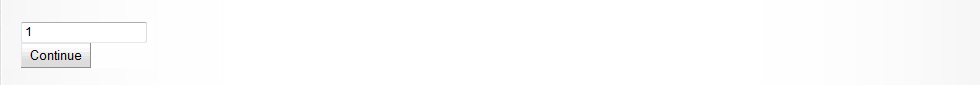
\includegraphics[scale=0.6]{img/examples/query.png}
%        \caption{}
%    \end{subfigure}
%	\begin{subfigure}[b]{1.0\textwidth}
%		\centering
%        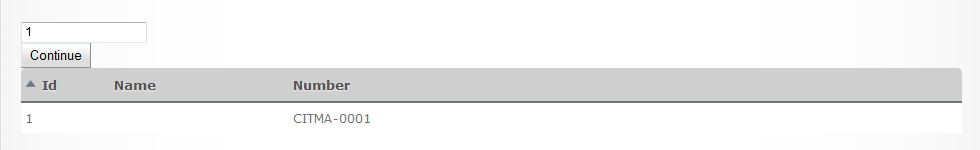
\includegraphics[scale=0.6]{img/examples/result.png}
%        \caption{}
%    \end{subfigure}
%    \caption{Sample page result}
%    \label{fig:sample_result}
%\end{figure}
%
%\subsubsection{Notes}
%This might seem like a lot of code, but remember that you don't have to create a new Service for each new request that you might have. You can just add a new method to the service we just defined for additional data that you need.\\
%\\
%Try to reuse services and service methods wherever you can to minimize code duplication.

\subsection{Internationalizing your pages}
\label{sec:example_i18n}
As already mentioned in Section \ref{sec:features_i18n}, Germinate supports internationalization for as many languages as you want.
Internationalizing your custom code is really easy:
\begin{enumerate}
    \item Define a method that returns your localized text in \path{jhi.germinate.client.i18n.Text}.
    \item Add the localized values for this new variable to the \texttt{.properties} files located at\\\instanceStuff\texttt{/<project.name>/modules/core/}. The file naming convention is: \texttt{Text\textunderscore\allowbreak <Language>\allowbreak \textunderscore <Region>.properties}.
\end{enumerate}
\noindent
A list of supported locales is available at \cite{JavaLocales}.

As an example, we will now add a new localized String to the application. To get the localized text, we used the method \texttt{Text.LANG.menuData()} which returned "data" for the English version of the page. Now let's assume we want to add a menu item that has the text "my fancy page". The first thing we have to do is create a new method in the interface \path{jhi.germinate.client.i18n.Text}:
\begin{lstlisting}[style=Java]
String menuMyFanyPage();
\end{lstlisting}
\noindent
As we can see, this method will return a \texttt{String} which we can use in our menu. You can regard this method as a template for the localization.\\
\\
The second step is to provide a translation of this text for each of the supported languages:
\begin{lstlisting}[style=Properties]
menuMyFanyPage=my fancy page
\end{lstlisting}
Add this to the files mentioned in the second bullet point above.\\
\\
GWT will substitute the template calls with the appropriate localized text during compile time.

\subsubsection{Parametrization and Plural Forms}
Instead of just returning static text from the properties files, Germinate is able to substitute place holders with parameters allowing for a dynamic usage of localization. One specific case of parameter usage is the case of plural forms. The text you want to display might differ based on the number of menus it should represent. As an example, consider the sentence: "I can see 3 trees". The sentence changes for just one tree: "I can see a tree". The method returning this text could look like this:

\begin{lstlisting}[style=Java]
String iSeeTrees(@PluralCount(DefaultRule_en.class) int number);
\end{lstlisting}
\noindent
The annotation \texttt{@PluralCount} tells the method that the parameter called \texttt{number} is a countable variable.
The associated properties entries could look like this:
\begin{lstlisting}[style=Properties]
iSeeTrees=I can see {0} trees.
iSeeTrees[one]=I can see a tree.
iSeeTrees[many]=I can see many trees.
\end{lstlisting}
As you can see, the plural form is handled by the first line, while the singular form is handled by the second line. A list of available plural forms can be seen in Table \ref{tab:examples_plural_form}. For more information, please refer to \cite{GWTPluralForms}.

\begin{table}
    \centering
    \caption{Available plural form rules in GWT}
    \label{tab:examples_plural_form}
    \begin{tabular}{rll}
	    \toprule
	    \textbf{Category} & \textbf{Rules} & \textbf{Examples}\\
	    \midrule
	    \textbf{zero} & $x$ is $0$ & 0\\
	    \textbf{one} & $x$ is $1$ & 1\\
	    \textbf{two} & $x$ is $2$ & 2\\
	    \textbf{few} & $x \bmod 100 \in \{3,...,10\}$ & 3-10, 103-110, \dots\\
	    \textbf{many} & $x \bmod 100 \in \{11,...,99\}$ & 11-99, 111-199, \dots\\
	    \textbf{other} & Everything else & 100-102, 200-202, 11.68, \dots\\
	    \bottomrule
    \end{tabular}
\end{table}

Another case of parametrization is simple substitution. As an example we will create a method returning a welcome message for the user and the day of the week.

\begin{lstlisting}[style=Java]
String welcomeMessage(String username, String day);
\end{lstlisting}
\noindent
The method is defined just the way a normal method taking two parameters would be defined. The localized entry in the properties file could look like this:

\begin{lstlisting}[style=Properties]
welcomeMessage=Hello {0}. Welcome to Germinate 3. Today is {1}.
\end{lstlisting}
\noindent
Calling \texttt{welcomeMessage("Joe Bloggs", "Wednesday");} will result in "Hello Joe Bloggs. Welcome to Germinate 3. Today is Wednesday".

\subsubsection{Notes}
\begin{itemize}
    \item It is possible to include HTML tags in the localized strings. Consequently, you can change the font style (size, bold, italic,...), add hyperlinks, include images, etc.
    \item Use two single quotes instead of just one (\eg "It''s done" instead of "It's done").
    \item The encoding of the properties files can be either UTF-8 or ISO-8859-1. If you choose the latter, make sure to encode all non-Latin-1 characters by using Unicode escape characters, \eg \textbackslash uXXXX where XXXX is the hexadecimal index of the character in the Unicode character set. A list of these characters can be found at \cite{Unicode}.
\end{itemize}

\subsection{Adding a new language}
\label{sec:i18n}
We have seen how to add content to existing languages in the previous section. Now we will show how to add a completely new language to the application. To ensure neutrality, we selected Switzerland and will use the language of Swiss German. The locale id of Swiss German is \texttt{de\textunderscore CH}. The first part represents the language (de = Deutsch which is German for "German") and the second part represents the country (CH = Confoederatio Helvetica which is Latin for "Swiss Confederation").

Navigate to your configuration folder located at \instanceStuff\texttt{/<project.name>} and create a new file called \texttt{Text\textunderscore de\textunderscore CH.properties}. Now copy the whole content of one of the fully translated other languages into this file and substitute all of the text with its appropriate translation.

Next, you'll need to make a change to this file: \path{war/css/language-selector-css.jsp}. Search for the line containing the 2-digit country code of the country associated with the new language. In our example, that would be \texttt{CH} and the line looks something like this:

\begin{lstlisting}[style=CSS]
span.country.ch { background-position: 0px -1440px; }
\end{lstlisting}
\noindent
Add a new line with your new locale before this line. Mind the comma:

\begin{lstlisting}[style=CSS]
.language-selector span.de_CH,
span.country.ch { background-position: 0px -1440px; }
\end{lstlisting}
\noindent
Finally, open the file \instanceStuff\texttt{/<project.name>/Germinate.gwt.xml} and add this line:

\begin{lstlisting}[style=Xml]
<extend-property name="locale" values="de_CH" />
\end{lstlisting}
\noindent
After compiling and deploying the project, you should be able to select the new localization from the language selector at the top of the page.

\subsubsection{Notes}
\begin{itemize}
    \item The default locale is determined by the browser settings. A fall-back solution can be specified by this entry in the \texttt{Germinate.gwt.xml} file:
            \begin{lstlisting}[style=Xml]
<set-property-fallback name="locale" value="en_GB" />
            \end{lstlisting}
    \item Not all localization files have to be complete. If translations are missing, they will be substituted by their respective value from the default locale.
\end{itemize}

\subsection{Internationalized files and images}
\label{sec:localized-files}
In some cases it may be necessary to supply a download file or image in more than just one language. We decided to adopt a concept called \textit{resource qualifiers}. This concept is also used in the popular Android platform \cite{ResourceQualifiers}.

The main idea of this concept is to provide resources in alternate forms which will be used under certain circumstances. On Android one example of a resource qualifier are language and region. Valid examples are \textit{de} for German resources or \textit{en-rGB} for British English.

The advantage of this concept is that you only have to copy your files/images to the appropriate folder and the system will choose the correct file based on the current configuration. If a file does not exist in the folder for the current configuration, the system will fall back to the default file.

We adopted this idea for Germinate. We allow internationalization of files in the directories "download", "data", and "res" (see Section \ref{sec:structure} for details). To provide internationalized versions of your files, you need to create a new directory of the type you want to extend (e.g. "download") and then append the locale separated by a dash. In the previous sections we used the local \texttt{de\textunderscore CH} as an example. The internationalized download directory for this locale would have to be named \texttt{download-de\textunderscore CH}. The structure within this directory has to be identical to the base-directory ("download"). Please note, that this concept only works if the files in the different directories have the same file name. Otherwise, Germinate won't be able to find them.

The result for the user is a seamless internationalization of all the content within Germinate. When changing the locale on the web interface, the server backend will serve the internationalized files for this locale, if available, and fall back to the default locale otherwise. 

\subsection{Using the \texttt{ParameterStores}}
The \texttt{TypedParameterStore} is an easy and convenient way to maintain a session state while navigating Germinate. This means that you can store selections the user makes on one page and reuse them on another page without having to pass them around. There is a typed version of the \texttt{TypedParameterStore} for each supported data type (\texttt{Long}, \texttt{String}, etc.). The important methods of the \texttt{ParameterStores} are:
\begin{lstlisting}[style=Java]
public static T get(Parameter key);
public static T set(Parameter key, T value);
\end{lstlisting}
The first method will return the saved values for the given parameter (if available) whereas the second method stores a new value for the given parameter. Note that the return type of \texttt{get()} is \texttt{T}, meaning that each sub-class returns the data in the suitable data type.

The list of available parameters is defined as the enum \path{jhi.germinate.shared.enums.Parameter}. New parameters can be added by simply adding a new value to the enum.

\subsubsection{Passing parameters via the URL}
When Germinate is first loaded by the browser, it will parse the given URL parameters and save the respective parameters in the \texttt{ParameterStores}. As a result, you can create URLs that take the user to a specific page for a specific combination of parameters. As an example, the URL
\begin{center}
\texttt{http://<your\textunderscore server>:8080/<project.name>/?accessionId=1\#passport}
\end{center}
will take you to the passport page of Germinate showing the accession with id 1. Alternatively, the URL
\begin{center}
\texttt{http://<your\textunderscore server>:8080/<project.name>/?searchString=Baz\#search}
\end{center}
will show the search results for the given search string. Multiple parameters can be specified by combining them with an ampersand (\&).\\
\\
For security reasons, we only save valid parameters, \ie parameters that are part of the enum \texttt{Parameter}. Moreover, it is very important that the parameters are located \textbf{before} the fragment identifier (\#).

\subsection{Using the notification system}
\label{sec:example_notification}
The Notification class (\path{jhi.germinate.client.util.Notification}) contains the following methods to create notifications:
\begin{lstlisting}[style=Java]
Notification.notify(Type.SUCCESS, "Message");

Notification.notify(Type.INFO, "Message");

Notification.notify(Type.WARNING, "Message");

Notification.notify(Type.ERROR, "Message");
\end{lstlisting}
\noindent
Methods taking two parameters allow using an arbitrary title, whereas methods with just one parameter will use the default title defined in the localized properties files.

%\subsection{Customizing the logo}
%\label{sec:example_logo}
%In this section, we will explain how to use a composite logo, that is, a logo consisting of multiple sub-logos. Figure \ref{fig:logo_example} shows an example of a logo composed of three sub-logos. Each of these logos will contain a link to the respective website.
%\begin{figure}
%    \centering
%    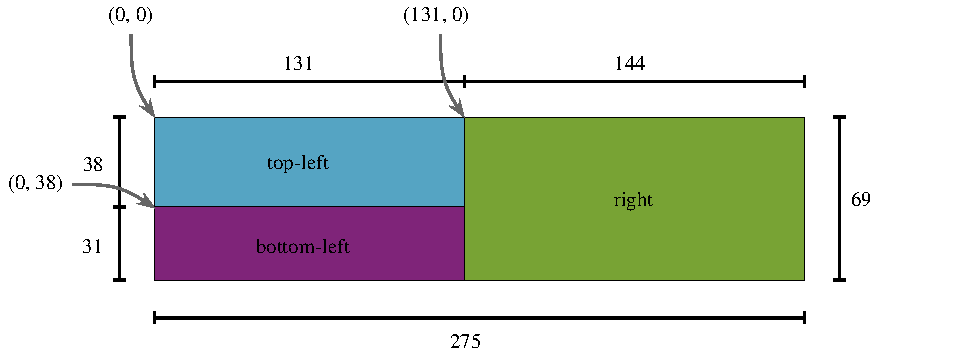
\includegraphics[scale=0.8]{img/examples/logo-example.pdf}
%    \caption{Logo example}
%    \label{fig:logo_example}
%\end{figure}
%
%To achieve this, we first define the three hyperlinks and assign ids to them. We will use the property \texttt{Germinate.Template.LogoMap} for this purpose (remember to keep everything in one line, we use multiple lines for better readability).
%
%\begin{lstlisting}[style=Properties]
%Germinate.Template.LogoMap=<a target="_blank" id="top-left" href="http://www.top-left.logo/"></a>
%                               <a target="_blank" id="bottom-left" href="http://www.bottom-left.logo/"></a>
%                               <a target="_blank" id="right" href="http://www.right.logo/"></a>
%\end{lstlisting}
%\noindent
%Now we can use the \texttt{css} file of your template to specify the size of each logo. Open the file \instanceStuff\texttt{/<project.name>/template/logo.css} and add the following lines to it:
%
%\begin{lstlisting}[style=CSS]
%#header {
%	height: 69px; /* Height of the header */
%}
%
%#logo {
%	width: 275px; /* Width of the logo */
%}
%
%#logo-image {
%	height: 69px; /* Height of the logo */
%}
%
%/* Settings for the top left logo part */
%#logo #top-left {
%	position: absolute;
%	top: 0px; /* Vertical start of the logo */
%	left: 0px; /* Horizontal start of the logo */
%	width: 131px; /* Width of the logo */
%	height: 38px; /* Height of the logo */
%	background-color: transparent;
%}
%
%#logo #bottom-left {
%	position: absolute;
%	top: 38px; /* Vertical start of the logo */
%	left: 0px; /* Horizontal start of the logo */
%	width: 131px; /* Width of the logo */
%	height: 31px; /* Height of the logo */
%	background-color: transparent;
%}
%
%#logo #right {
%	position: absolute;
%	top: 0px; /* Vertical start of the logo */
%	left: 131px; /* Horizontal start of the logo */
%	width: 144px; /* Width of the logo */
%	height: 69px; /* Height of the logo */
%	background-color: transparent;
%}
%\end{lstlisting}
%\noindent
%The first three styles specify the overall size of the composite logo whereas the last three styles specify the individual sizes. Look at Figure \ref{fig:logo_example} again to see where each number comes from. Change the values according to your logo and save the file.
%
%Finally, place your composite logo in the \texttt{template} folder and deploy the application.

\subsection{Using D3.js}
D3.js \cite{D3} (D3 for Data-Driven Documents) is a JavaScript library used to create interactive data visualizations in the browser backed by Scalable Vector Graphics (SVG). D3.js is a highly complex framework and creating new charts can be tricky at times. This is why we integrated reusable versions of a set of frequently used chart types into Germinate. Those include: scatter plots, histograms, bar charts, line charts, treemaps, etc.

Using these reusable charts is straightforward. In this section, we will create a scatter plot as an example. The following code snippet is used to create the chart:

\begin{lstlisting}[style=JavaScript, numbers=left, numbersep=5pt, numberstyle=\tiny\color{gray}, escapechar=|]
d3.tsv('scatter-plot.tsv', function (data) { |\label{code:d3-tsv}|
    d3.select('#scatter-plot') |\label{code:d3-select}|
        .datum(data) 
        .call(scatterPlot() |\label{code:d3-scatter-plot}|
            .margin(margin) |\label{code:d3-margin}|
            .width(width)
            .height(height) |\label{code:d3-height}|
            .x(function (d) { return parseFloat(d.x); }) |\label{code:d3-x}|
            .y(function (d) { return parseFloat(d.y); }) |\label{code:d3-y}|
            .colorKey(function (d) { return d.name; }) |\label{code:d3-color}|
            .tooltip(function (d) { return d.name + '<br/>(' + d.x + ', ' + d.y + ')'; }) |\label{code:d3-tooltip}|
            .onClick(function (d) { console.log(d); }) |\label{code:d3-click}|
            .showDistribution(true) |\label{code:d3-distribution}|
            .xLabel('weight [g]') |\label{code:d3-x-label}|
            .yLabel('diameter [mm]') |\label{code:d3-y-label}|
        );
});|\label{code:d3-count}|
\end{lstlisting}
\noindent
Now, let's explain what this code actually does. In line \ref{code:d3-tsv}, we tell D3.js to load a file called \texttt{scatter-plot.tsv} (see Table \ref{table:d3-input-data}). A \texttt{tsv} file is a file of tab-separated values (like a \texttt{csv} only with tabs instead of commas). The result is passed to the following function as the variable \texttt{data}.

In line \ref{code:d3-select}, we select the HTML element with the id "\texttt{scatter-plot}", then use our data on this element and call the function \texttt{scatterPlot}. The code so far would be enough to create a scatter plot if our data was formatted in the format expected by the reusable chart. Lines \ref{code:d3-margin} to \ref{code:d3-height} define the margin, width and height of the chart. Please note, that we omitted the definition of these variables here. Width and height are integer values, whereas margin is an object containing the values \texttt{top}, \texttt{right}, \texttt{bottom} and \texttt{left}. Lines \ref{code:d3-x} and \ref{code:d3-y} tell the chart how to extract the values for x and y axis respectively. As you can see, they use \texttt{d.x} and \texttt{d.y} as the values are defined in the x and y columns of the input file. Line \ref{code:d3-color} is used to define which column of our input data should be used to determine the color of the data point. In this example, we want all the points of the same accession to have the same color. The accession name is defined in column \texttt{name}, so we return it. Line \ref{code:d3-tooltip} extracts the information to show inside the tooltip when the user hovers over the data point. Line \ref{code:d3-click} can be used to implement on-click behaviour. This could be a simple popup message or a completely new page with additional information about the clicked element. Line \ref{code:d3-distribution} enables the distribution visualization along the sides. Lines \ref{code:d3-x-label} and \ref{code:d3-y-label} define the axis titles for x and y axis respectively.\\
\\
Using just these \ref{code:d3-count} lines, we can create the interactive scatter plot shown in Figure \ref{fig:d3}. Just to put this number into context: The implementation of the reusable \texttt{scatterPlot} function is roughly 350 lines long. This, however, includes a multitude of configuration options that aren't used in this example.

\begin{table}
	\caption{Input data}
	\label{table:d3-input-data}
	\centering
	\begin{tabular}{cccc}
		\toprule
		\textbf{id} & \textbf{name} & \textbf{x} & \textbf{y}\\
		\midrule
		3 & CACTUAR-000005 & 4.08695 & 0.465969 \\
		3 & CACTUAR-000005 & 3.55 & 0.451295 \\
		3 & CACTUAR-000005 & 4 & 0.452107 \\
		3 & CACTUAR-000005 & 3.7 & 0.474437 \\
		$\vdots$ & $\vdots$ & $\vdots$ & $\vdots$\\
		\bottomrule
	\end{tabular}
\end{table}

\begin{figure}
	\centering
	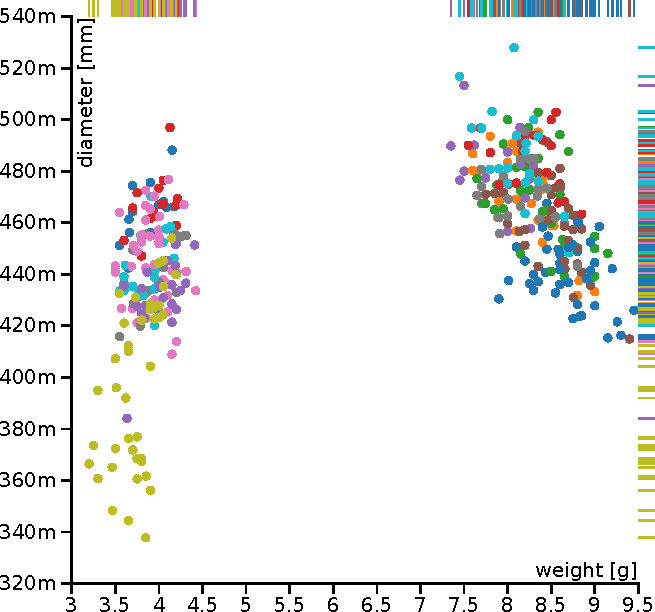
\includegraphics[width=0.5\textwidth]{img/examples/d3.pdf}
	\caption{D3.js scatter plot}
	\label{fig:d3}
\end{figure}

\subsection{Important notes}
We try our best to make Germinate as secure as possible. The code you download from our page has been tested intensively to ensure that your data and your users are safe and secure.

That said, Germinate is only as secure as its individual parts. Should you decide to extend Germinate and add your own code to it, it is in your responsibility to ensure the security of your version of Germinate.

In this section, we will explain what types of security/safety issues can arise when developing with GWT and JavaScript and we will cover solutions for the most common issues. Please refer to the official documentation \cite{GWTSecurity} for a complete list.

\subsubsection{XSS and GWT}
Cross-site scripting (XSS) is a security vulnerability that enables attackers to inject malicious scripts into the web page. GWT prevents XSS very well \textbf{if used correctly}. XSS can be avoided if you follow good JavaScript coding practices. Here is a list of things to keep in mind:

\begin{description}
	\item[Avoid using \texttt{new HTML(String)} and \texttt{HTML\#setText(String)}]\hfill \\The class \texttt{com.google.gwt.user.client.ui.HTML} is a popular way of adding HTML code in the form of a \texttt{String} to your page. This is perfectly fine if you know where the \texttt{String} came from and what it contains, or in other words, if you are certain that the \texttt{String} doesn't contain malicious code. However, if the \texttt{String} is passed down to your code as a parameter and you don't know it's origin, this may entail a security issue.
	
	There are ways to prevent this, however:
	\begin{itemize}
		\item Prefer plain-text widgets, \eg \texttt{Label}. If your text does not contain HTML tags, it's preferable to use a \texttt{Label} instead.
		\item Change your parameter type from \texttt{String} to \texttt{SafeHtml}. \texttt{SafeHtml} represent XSS-Safe HTML and it's therefore safe to use it. The easiest way to use \texttt{SafeHtml} is to change the return type of the internationalization methods seen in Section \ref{sec:example_i18n} from \texttt{String} to \texttt{SafeHtml}. Refer to the official documentation to find out how to create instances of \texttt{SafeHtml} without this approach.
	\end{itemize}
	\item[Avoid using the JavaScript function \texttt{eval()} in JSNI methods]\hfill \\The JavaScript Native Interface (JSNI) allows you to define JavaScript code embedded in Java code. This can be useful in cases where the default GWT implementation just doesn't provide the JavaScript functionality you require. When using JSNI, you of course can't rely on GWT to take care of XSS prevention. Consequently, be very careful when using JSNI. One of the most common mistakes is calling the JavaScript function \texttt{eval()}. This function takes a \texttt{String} and executes it as if it were regular JavaScript. This already screams "Security Issue".
	\item[Avoid code that sets \texttt{innerHTML} of GWT widgets]\hfill \\This is related to the first item in this list. Manipulating \texttt{innerHTML} of GWT widgets circumvents the XSS security mechanisms of GWT and therefore is not recommended. Setting \texttt{innerText} (plain-text) on the other hand is safe.
\end{description}

\subsubsection{XSRF and GWT}
Cross-Site Request Forgery (XSRF) is a type of attack where the attacker can perform actions on behalf of a verified user without the user's knowledge. The attacker uses the valid user session to start these requests to the server. Without any further measures, JavaScript and therefore GWT are vulnerable to XSRF attacks.

However, we included a mechanism in Germinate that prevents XSRF attacks. This mechanism requires you to send the session id with \textbf{every} request sent to the server. The server can then verify this session id (token) against the actual id of the session and the cookie. Only if all three ids are identical will Germinate return the requested data or execute the query. This security mechanism has already been covered in detail in Section \ref{sec:example_security}.





